\documentclass{goose-article}

\setcounter{topnumber}{2}
\setcounter{bottomnumber}{2}
\setcounter{totalnumber}{4}
\renewcommand{\topfraction}{0.85}
\renewcommand{\bottomfraction}{0.85}
\renewcommand{\textfraction}{0.15}
\renewcommand{\floatpagefraction}{0.8}
\renewcommand{\textfraction}{0.1}
\setlength{\floatsep}{5pt plus 2pt minus 2pt}
\setlength{\textfloatsep}{5pt plus 2pt minus 2pt}
\setlength{\intextsep}{5pt plus 2pt minus 2pt}

\title{The Five `D''s of Friction -- Final Report}
\author{Tom de Geus}
\hypersetup{pdfauthor={T.W.J. de Geus}}

\begin{document}

\twocolumn[
    \begin{@twocolumnfalse}
        \maketitle
    \end{@twocolumnfalse}
]
\sloppy

\section{Project goal}

\paragraph{Background}

When a frictional interface is driven quasistatically, periods of loading are punctuated by sudden macroscopic slip events.
Field observations on earthquakes and laboratory studies support that slip nucleates at weak regions of the interface and then propagates ballistically as a fracture.
Understanding under which conditions large slip events are triggered and can propagate is central to tribology, for example to explain the observed variability of friction coefficients, and for earthquake science.

\paragraph{Goal}

The goal of this project was to understand which collective microscopic dynamics are responsible for the nucleation of slip events at frictional interfaces, and develop a theoretical prediction for the stick-slip amplitude.
This goal is achieved, as summarised below.
New open questions are also identified.

\paragraph{Note to reader}

This report summarizes the main results of the project.
It includes citations to the publications that have resulted from the project.
References to other literature are not included, but can be found in the cited publications.

\section{State-of-the-art}

\paragraph{Friction coefficient}

It is well known that the shear force required to initiate slip is proportional to the normal force on the object.
Since friction is in addition independent of the nominal contact area, one should study the \emph{shear stress}.
In all of the following, we uniquely study the shear stress.
We denote $f$ the remotely applied shear stress (proportional to the force with one needs to pull a sliding block).
For simplicity, we will refer to $f$ as force and not that our results are on non-dimensional (and could be converted to desired units if needed).

\paragraph{Continuum models}

On a macroscopic level, experiments on a wide variety of materials support that the frictional response is velocity-weakening.
Many experiments are well described by rate-and-state friction models.
Concrete ideas about the nucleation of slip have been developed by studying the stability of a perturbation of a stable interface subject to homogeneous rate-and-state models.
These works predict that a perturbation of extent $\ell$ is unstable if $\ell > \ell_c \sim (f - f_c)^{-1}$.
\emph{However, the microscopic collective dynamics that form the perturbation remain unclear.}

\paragraph{Roughness}

Zooming in on the interface, it is well known that any interface is rough.
At any instance of time, a fraction of local hills forms a contact that elasticity resists deformation up a certain threshold to local ``failure''.

\paragraph{Disordered models}

We can model such phenomenology as an elastic interface driven over a disordered pinning potential using a weak spring.
The elasticity accounts for the fact that points along the interface cannot slip independently.
The disorder accounts for the fact that contacts elastically resist deformation up to a local (`random') threshold.

\paragraph{Depinning transition}

If overdamped dynamics are considered, such models undergo a depinning transition at a critical force $f_c$.
At $f_c$, the interface moves via large reorganizations, called avalanches.
Their size is power law distributed, $P(S) \sim S^{-\tau_\mathrm{dep}}$.
Moreover, the interface shape is a self-similar shape with a roughness exponent $\zeta_\mathrm{dep}$.
At lower applied forces ($f < f_c$), the avalanche's maximal linear extent diverges approaching the critical point: $\ell_\mathrm{dep} (f) \sim |f - f_c|^{-\nu_\mathrm{dep}}$.
At higher applied forces ($f > f_c$) the interface moves at a finite velocity.
The exponents $\tau_\mathrm{dep}, \zeta_\mathrm{dep}, \nu_\mathrm{dep}, \ldots$ are now well understood and related by scaling relations.
A practical note thereby that the roughness exponent $\zeta_\mathrm{dep}$ captures the spatial correlations of slip.
This is a priori unrelated from the surface roughness of the frictional interface, that is captured the physical height-height correlations of the interface.
\emph{Crucially, the depinning transition is a continuous transition: it does not display stick-slip as observed at the frictional interface and in earthquakes.}

\section{Key physics: inertia}

\paragraph{Finite mass}

The key physics to link the macroscopically observed stick-slip (due to velocity-weakening) to the microscopic collective dynamics of the interface, is inertia.
At the frictional interface local failure corresponds to the failure of ``asperities'' (hills) of a finite size and mass.
Moreover, the elastic bulk permits elastic wave propagation.

\paragraph{Intuition}

The effect of inertia can be understood as follows.
During elastic loading the interface climbs up energy barriers, but then abruptly slides downhill once the barrier is overcome.
For overdamped systems (that display the continuous depinning transition), this descent suffices to dissipate the energy stored during loading, while at lower damping the inertia may carry the system over several successive barriers leading to force overshoots and oscillations.
Such oscillations emit acoustic waves that facilitate failure of neighbouring regions.
Since their failure also emits waves, there is a feedback corresponding to velocity-weakening.

\paragraph{Rheololgy}

The remote force $f$ is a combination of the velocity-weakening of the interface and dissipation.
The resulting flow curve is non-monotonic, with a minimum at $f = f_{\min}$, as sketched in \cref{fig:nonmonotic:a}.

\paragraph{Stick-slip}

If an inertial interface is driven quasistatically through a weak spring\footnote{
    The interface is connected to a loading frame using a weak spring.
    Quasistatic loading corresponds to increasing the position of the driving frame infinitely slowly, such that energy is minimised at each step.
    In the context of the frictional interface, the elastic bulk plays the role of the weak spring, with the effective stiffness proportional $1 / H$, with $H$ the height of the block.
}, ``stick-slip'' occurs as sketched in \cref{fig:nonmonotic:b}.
The main question is now to understand the amplitude of the slip events.

\begin{figure}[htp]
    \subfloat{\label{fig:nonmonotic:a}}
    \subfloat{\label{fig:nonmonotic:b}}
    \centering
    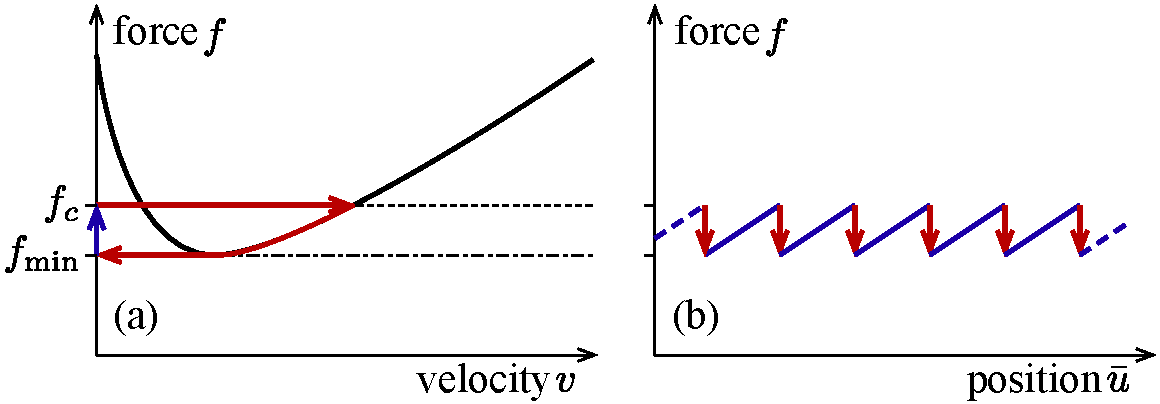
\includegraphics[width=\linewidth]{figures/theory_homogeneous.pdf}
    \caption{
        [Sketch] \protect\subref{fig:nonmonotic:a} With inertia the flow curve (force $f$ \emph{vs} velocity $v$) is non-monotonic, with a minimum at $f = f_{\min}$.
        \protect\subref{fig:nonmonotic:b}
        A finite hysteresis is predicted in the thermodynamic limit, such that a system driven quasistatically through a weak spring displays stick-slip.
        Thereby, power law distributed avalanches protect the interface from building up a load $f > f_c$ where it is unstable.
        After the instability, the interface unloads to $f = f_{\min}$ while slipping (see corresponding cycle in panel \protect\subref*{fig:nonmonotic:a} with the same colour coding).
    }
    \label{fig:nonmonotic}
\end{figure}

\section{Main result}

\paragraph{Nucleation}

We propose that, in the presence of disorder, avalanches constitute to the perturbations that nucleate slip events.
In particular, for quasistatic loading using a weak spring, we find criticality at $f_c$, such that the avalanche size, extent, \dots, are distributed according to power laws.
Furthermore, we find that an avalanche is unstable if its extent $\ell > \ell_c \sim (f - f_c)^{-\nu}$~\cite{deGeus2022,deGeus2024a}.
In an infinitely large system, the interface is thus protected from building up a load $f > f_c$.
If an instability occurs, the system advances by a large reorganization, and unloads to $f_{\min}$ (the minimum of the flow curve), resulting in the stick-slip cycle in \cref{fig:nonmonotic}.
Thereby we numerically find that $f_c \approx f_{\min}$ in very large systems \cite{deGeus2022,deGeus2024a,deGeus2019}.
Crucially, the disorder is responsible for a distribution of barriers resulting in a self-affine roughness of the interface characterized by an exponents $\zeta$, which can be related to criticality to the non-trivial exponent $\nu$.
Thereby, we find that all exponents and most of their scaling is different from the depinning transition.
Moreover, we find that the nucleation of slip at a disordered interface is not captured by continuum theory.

\paragraph{Armouring}

In a finite system, the stick-slip amplitude is increased due to armouring by inertia \cite{deGeus2019,ElSergany2023}.
In particular, we find that if the interface stops after a system spanning event there are very few regions with a small activation energy in the forward direction.
Consequently, the number of avalanche is reduced, such that the interface can build up a load $f_s > f_c$, \cref{fig:pre:flow,fig:pre:stick-slip}.
The scarcity of avalanches thereby masks the criticality of the interface, as a bimodal event size distribution is observed instead, see \cref{fig:pre:bimodal}, indeed argued to be the distribution of earthquakes on a single fault.
To study the properties of avalanches in an infinite system, we trigger avalanches at different forces $f$ and study their statistics.
At $f_c$, their properties are scale free.
At $f > f_c$, avalanches transition to system spanning events if their extent $\ell > \ell_c$, see \cref{fig:pre:ellc}.
We predict and test $f_s - f_c$ as a function of the system size and the exponents $\tau$, $\nu$, and that of the distribution of activation barriers.

\begin{figure}[htp]
    \subfloat{\label{fig:pre:flow}}
    \subfloat{\label{fig:pre:stick-slip}}
    \subfloat{\label{fig:pre:bimodal}}
    \subfloat{\label{fig:pre:ellc}}
    \centering
    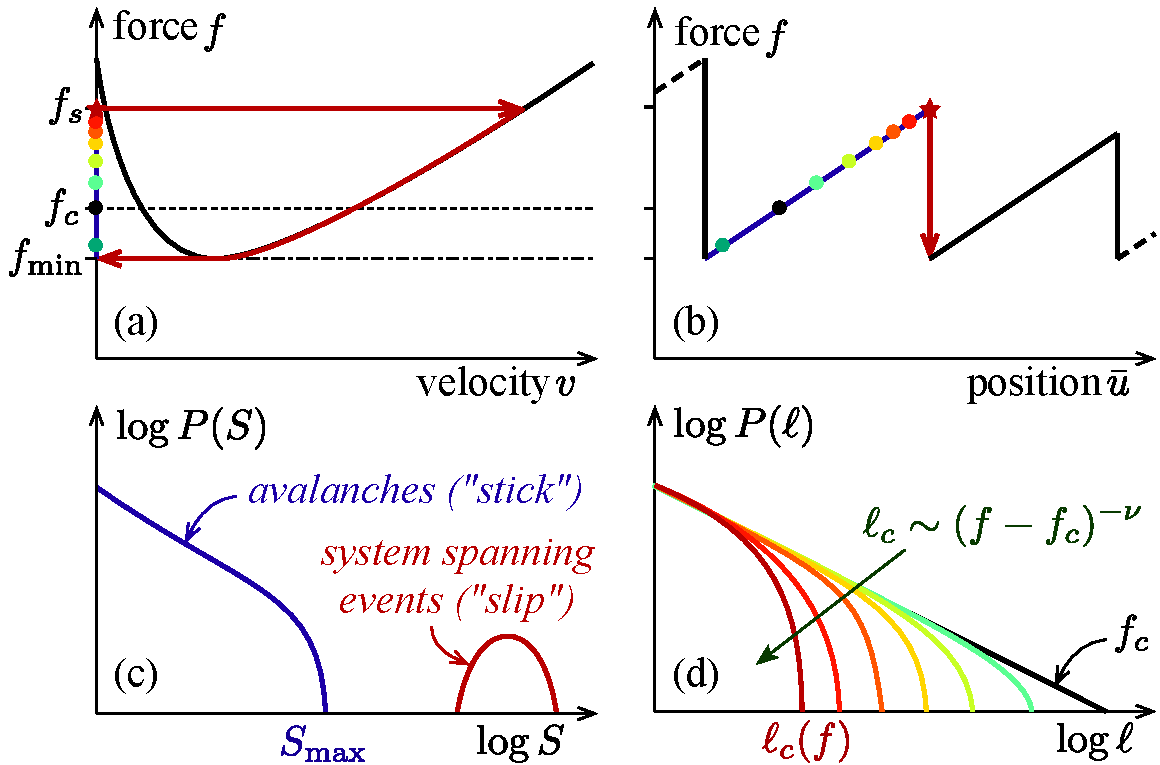
\includegraphics[width=\linewidth]{figures/theory.pdf}
    \caption{
        [Sketch] (\protect\subref*{fig:pre:flow}-\protect\subref*{fig:pre:stick-slip}) In a finite system with disorder, avalanches occur at any force $f \geq f_{\min}$.
        They nucleate slip once their extent $\ell > \ell_c \sim (f - f_c)^{-\nu}$, typically at $f = f_s$.
        \protect\subref{fig:pre:bimodal} The corresponding distribution of event sizes, $P(S)$, during a quasistatic cycle is bimodal, see panel \protect\subref*{fig:pre:bimodal}, with avalanches up to a scale $S_{\max}(f_s)$, and system spanning events at a much bigger scale.
        \protect\subref{fig:pre:ellc} To study the properties of avalanches in an infinite system, and to quantify $\ell_c$, we trigger avalanches at different forces $f$.
        The distribution of their linear extent $\ell$ is scale free at $f_c$ while at $f > f_c$ avalanches transition to system spanning events if $\ell > \ell_c$ (system spanning events are excluded from the shown distributions).
    }
    \label{fig:pre}
\end{figure}

\section{The five `D''s of friction}

\paragraph{Disorder}

Disorder changes the distribution of activation barriers after a system spanning event.
In particular, let $P(x)$ the density of microscopic regions that fail if the shear load is increased by some amount $x$.
If $P(x)$ vanishes at small argument as $P(x)\sim x^\theta$ \cite{deGeus2019}, then increasing the load by $\Delta f$ triggers a finite number of avalanches, proportional to $(\Delta f)^{\theta+1}$.
The exponent $\theta$ is nonzero only in the presence of inertia (otherwise $\theta=0$).
It was found to depend on the statistics of the disorder \cite{deGeus2019}.
A single-particle toy model with inertia and disorder captures the existence of a non-trivial exponent $\theta>0$, which we can analytically relate to the statistics of the disorder \cite{ElSergany2023}.
\emph{Future work should clarify quantitative discrepancies between the theory and measurements.}
\emph{Moreover, crucially, future work should relate the physical surface roughness of the frictional interface to the statistics of the disorder.}

\paragraph{Dissipation}

In a $d$ dimensional interface embedded in a $d + 1$ dimensional elastic medium, on top of damping due to thermalisation, the inertia of the medium has a stabilization effect known as ``radiation damping''.
This changes stick-slip if a system has very weak background damping, for example because only little energy is lost at the system's boundaries.
Suppose that the resistance of the pinning potential as a function of velocity is $f^p(v)$.
Then, during flow, the remote force $f$ measured at the system's boundaries is $f = f^p(v) + \eta v$, with $\eta$ the background damping, see \cref{fig:radiation:b}.
A nucleating event, whereby part of the interface and bulk are still static as the rupture invades the interface, is stabilized by the bulk surrounding it: to increase the velocity $v$, the bulk around the rupture has to be accelerated.
The costs of this acceleration lead to a remote force $f = f^p(v) + (\mu / (2 c_v)) v$, with $\mu$ the shear modulus of the bulk, and $c_s = \sqrt{\mu / \rho}$ the shear wave speed of the bulk, with $\rho$ the mass density of the bulk, see \cref{fig:radiation:a}.
Because the bulk is accelerated by elastic waves that radiate away from the interface this effect is commonly referred to as ``radiation damping''.

In the case that $\eta \ll \mu / (2 c_v)$ the stick-slip cycle of a thermodynamic system is now as follows.
During nucleation, the net velocity of the interface is zero, and the flow curve is stabilized by radiation damping with a minimum at $f_{\min}^\text{nucl}$, see \cref{fig:radiation:a}.
As above, slip starts if $f = f_c > f_{\min}^\text{nucl}$.
Once moving, the radiation damping term disappears and the flow curve is lowered with a minimum at $f_{\min}^\text{flow}$, see \cref{fig:radiation:b}.
The system thus stops if $f = f_{\min}^\text{flow} < f_{\min}^\text{nucl} < f_c$.
This corresponds to the stick-slip cycle shown in \cref{fig:radiation:c,fig:radiation:d}.

We expect criticality to be observed at $f = f_c$.
As before, we expect an instability if an avalanche's extent $\ell > \ell_c \sim (f - f_c)^{-\nu}$.
However, by the same argument, we expect avalanches at $f < f_c$ to be sub-extensive such that the distribution of their extent $P(\ell)$ is cut off at $\ell_c \sim (f - f_c)^{-\nu}$ for which we expect the same exponent to hold.
We qualitatively confirmed this picture using the model of \cite{deGeus2019,deGeus2022}, but lack a quantitative confirmation, \emph{which is left for future work}.

\begin{figure}[htp]
    \subfloat{\label{fig:radiation:a}}
    \subfloat{\label{fig:radiation:b}}
    \subfloat{\label{fig:radiation:c}}
    \subfloat{\label{fig:radiation:d}}
    \centering
    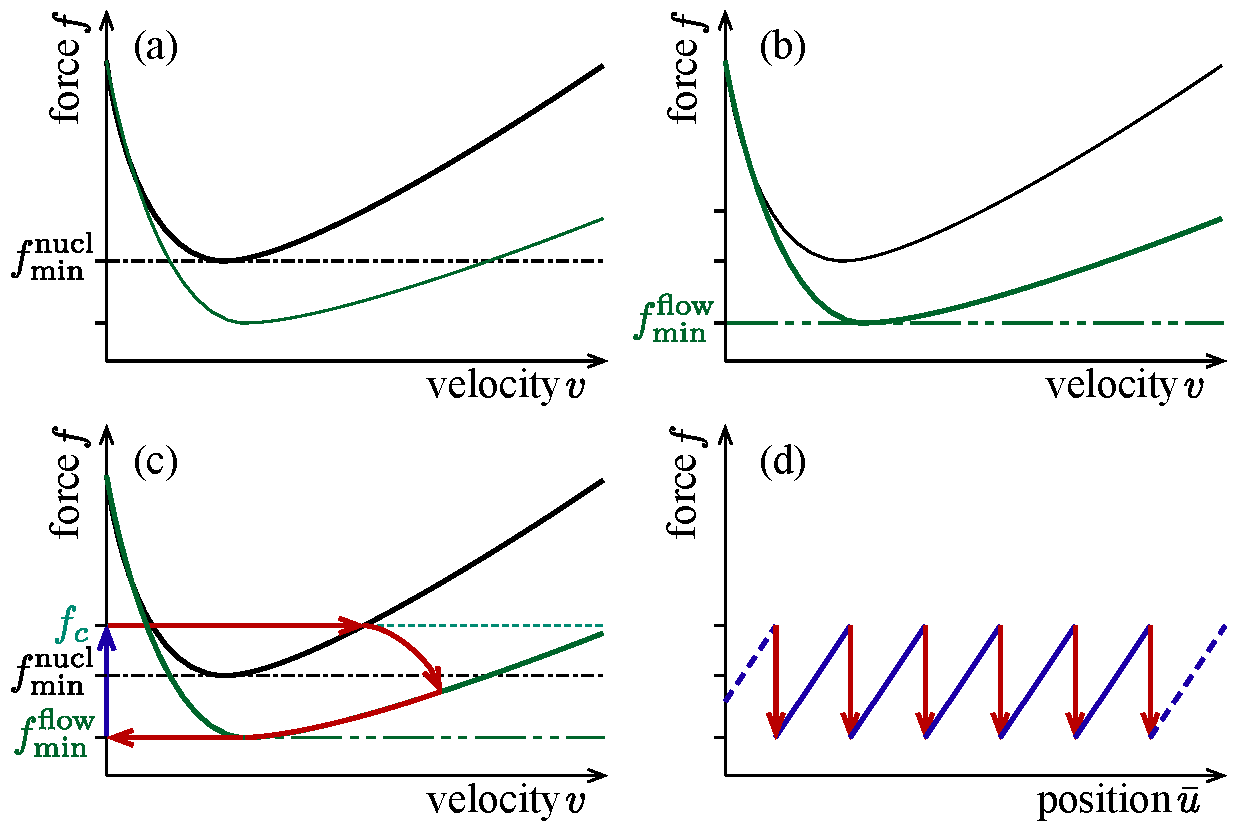
\includegraphics[width=\linewidth]{figures/radiation_damping.pdf}
    \caption{
        [Sketch] In a $d$ dimensional interface embedded in a $d + 1$ dimensional elastic medium, on top of damping due to thermalisation, also the inertia of the medium has a stabilization effect known as ``radiation damping''.
        For low background damping, this can lead to an additional source of hysteresis.
        \protect\subref{fig:radiation:a} During nucleation, the background damping is dominated by radiation damping leading to a non-monotonic flow curve with a minimum at $f_{\min}^\text{nucl}$.
        \protect\subref{fig:radiation:b} Once moving, the radiation damping term disappears and the flow curve is lowered with a minimum at $f_{\min}^\text{flow}$.
        (\protect\subref*{fig:radiation:c},\protect\subref*{fig:radiation:d}) Quasistatic loading of the interface in the thermodynamic limit results in stick-slip whereby slip nucleates at $f_c > f_{\min}^\text{nucl}$ and stops at $f_{\min}^\text{flow} < f_{\min}^\text{nucl} < f_c$, as indicated with arrows and corresponding colours.
    }
    \label{fig:radiation}
\end{figure}

\paragraph{Drive}

Stick-slip is observed when driving with a weak spring.
Making this spring more rigid can suppress stick-slip if the stiffness is larger than a critical value.
This fact has been used to measure the non-monotonic rheololgy from \cref{fig:nonmonotic:a} \cite{deGeus2024a}.

\paragraph{Dimensionality}

Dimensionality changes the critical exponents.
In particular, we found that the value of the exponents $\tau$, $\nu$, \dots, are different for short-range \cite{deGeus2024a} and long-range depinning \cite{deGeus2022}.
Both studies we performed for a $d = 1$ dimensional interface.
The theoretical prediction was confirmed for a $d = 2$ dimensional interface with short-range depinning \cite{deGeus2024b}.
However, due to the computational costs, a definitive confirmation is left for future work.

\paragraph{Delay}

At a finite temperature, the interface experiences slow creep dynamics.
This qualitatively changes the stick-slip response of a stack of slabs in contact through dry frictional interfaces driven in quasistatic shear \cite{Poincloux2023}.
A lower driving stiffness the slabs slip asynchronously and, experimentally, to the stick-slip amplitude becoming broadly distributed as the number of layers in the stack increases.
We interpret this broadening in light of the combined effect of complex loading paths due to the asynchronous slips and creep.
Consequently, the aging rate of the interfaces can be readily extracted from the stick-slip cycles, and it is found to be of the same order of magnitude as existing experimental results on a similar material.

To fundamentally understand the creep dynamics, we first study the response of the interface at a small force, where the effect of inertia is negligible, and finite temperature.
At small forces, creep proceeds via thermal avalanches of activated events.
Due to elastic coupling, the thermal activations are spatially correlated: thermal avalanches occur.
We predict the exponents of thermal avalanches to be the same exponents as the depinning transition itself \cite{deGeus2024}.
\emph{With inertia, creep and elastic instabilities are expected to co-exist at forces of the order of $f_c$, how this qualitatively and quantitatively changes the stick-slip response is a fundamental open question.}

\section{Front dynamics}

We numerically confirmed that the front an unstable avalanche is fracture-like, and thus well understood by the theory of fracture.
Before the instability, the front of the avalanche is fractal.
Its dynamics are predicted by a scaling argument that combines the exponents of the avalanche with the finite velocity $v_{\min}$ if the interface is driven at $f_c \approx f_{\min}$~\cite{deGeus2022}.

\section{Supporting work}

Some of the properties of an elastic interface driven over a disordered pinning potential are strongly related to the plasticity of amorphous materials.
To better understand these parallels, joint studies were performed on: the nucleation of a thin shear band \cite{Popovic2018}, creep flow \cite{Popovic2021b,Popovic2021a}, and the distribution of activation barriers \cite{Ji2022,Ji2020,Ji2019}.

In addition, to support the research community in general, best practices of numerical simulations were shared \cite{deGeus2023}.

\bibliographystyle{unsrtnat}
\bibliography{library}

\end{document}
